\subsection{原理}
在课上的假设2(线性条件)和假设3(X的条件方差是常矩阵)条件成立下,有:
\begin{align*}
    &H_1 = \Sigma_{XXY}  \\
    &span(H_1) \subseteq S_{Y|X} \\
    &H_2 = E[(Y-E(XY)^TX)XX^T] \\
    &span(H_2) \subseteq S_{Y|X}
\end{align*}
\subsection{样本计算流程}
\begin{enumerate}
    \item 将$X_1,\dots,X_n$标准化为$Z_1,\dots,Z_n$
    \item 计算$\hat{\Sigma}_{ZZY}E_n(ZZ^TY),\quad \hat{\Sigma}_{XX}Var_n(X)$
    \item 计算$\hat{\Sigma}_{ZZY}$的前$q$个特征向量$u_1,\dots,u_n$,则对$S_{Y|X}$中向量的估计为$v_k=\hat{\Sigma}_{XX}^{-1/2}u_k,k=1,\dots,q$
\end{enumerate}

\subsection{度量两空间间的距离}
采用$L_2-Hausdorff$子空间距离度量$m$维子空间$U$与$n$维子空间$V$之间的距离:
$$d(U,V)=max(\vec{d}(U,V),\vec{d}(V,U))=\sqrt{max(m,n)-\sum_{i=1}^m\sum_{j=1}^n(u_i^Tv_j)^2}$$

在pHd方法中,选取了y对x的线性回归模型、泊松回归模型、logistics回归模型与cos函数关系来观察pHd方法的降维效果。结果也可以看处,
\subsection{线性回归}
设定样本量为1000,样本$X$维度为$5$,X每一维度上的值均从标准正态分布中取样。$\beta$作用X降维后的维度为$2$.即$\beta$是10*2的矩阵。一次的计算结果$H_1,H_2$如下表所示。设定的真实的$\beta$如下
\begin{equation}       %开始数学环境
   \beta= \left(                 %左括号
      \begin{array}{cc}   %该矩阵一共3列,每一列都居中放置
        1 & 0 \\  %第一行元素
        0 & 1 \\  %第二行元素
        0 & 0 \\
        0 & 0 \\
        0 & 0 \\
      \end{array}
    \right)                 %右括号
\end{equation}

\begin{table}[htbp]
\centering
\caption{线性回归结果}
\label{tab:norm}
\begin{tabular}{l|l|ll}
\hline
\multicolumn{2}{c|}{$H_1$} & \multicolumn{2}{c}{$H_2$}                    \\ \hline
$\hat{\beta_{1}}$&$\hat{\beta_{2}}$& \multicolumn{1}{l|}{$\hat{\beta_{1}}$}  &$\hat{\beta_{2}}$ \\ \hline
-0.7193995  & 0.07794245   & \multicolumn{1}{l|}{0.6920215}  & 0.4112301  \\ \hline
-0.2187786  & -0.24974545  & \multicolumn{1}{l|}{-0.1080706} & -0.7261988 \\ \hline
-0.5618548  & 0.28103448   & \multicolumn{1}{l|}{0.6192357}  & -0.3741050 \\ \hline
-0.1909770  & -0.92664516  & \multicolumn{1}{l|}{-0.2790291} & 0.2171582  \\ \hline
-0.3313467  & -0.03092594  & \multicolumn{1}{l|}{-0.2530621} & 0.2974159  \\ \hline
\end{tabular}
\end{table}
表\ref{tab:norm}可以看出,与真实的参数$\beta$相比,phd用H1方法得到的结果,并不是很接近。而且在降维后的维度不变情况下,随着X本身维度增加,估计效果越不好。
接下来判断维度的增大对降维效果的影响,设定$X$维度依次为$3-20$,统一降维至二维,采用H1方法,估计$\beta$,重复实验100次,计算距离的均值。判断依据为两个空间的距离($L_2-Hausdorff$子空间距离,越接近0表示两个空间越接近).如下图所示
\begin{figure}[H]
    \centering
    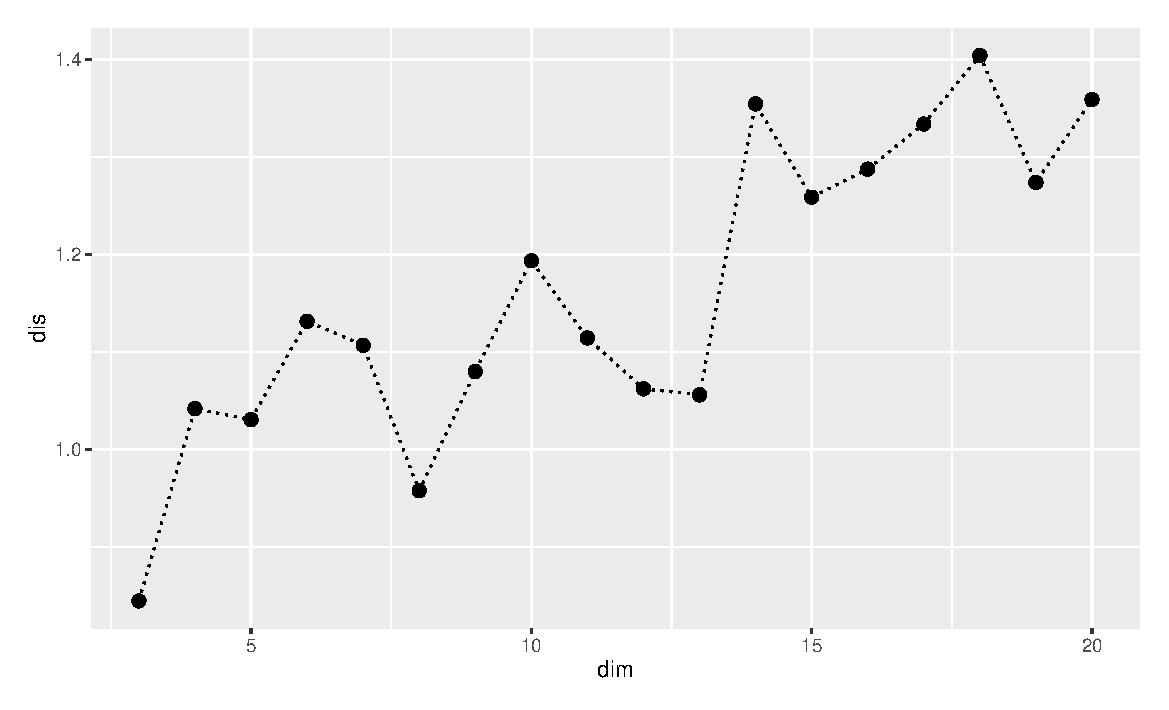
\includegraphics[width=0.8\textwidth]{image/norm.eps} 
    \caption{线性回归下维度对降维效果的影响}
\end{figure}


\subsection{泊松回归}
\begin{figure}[H]
    \centering
    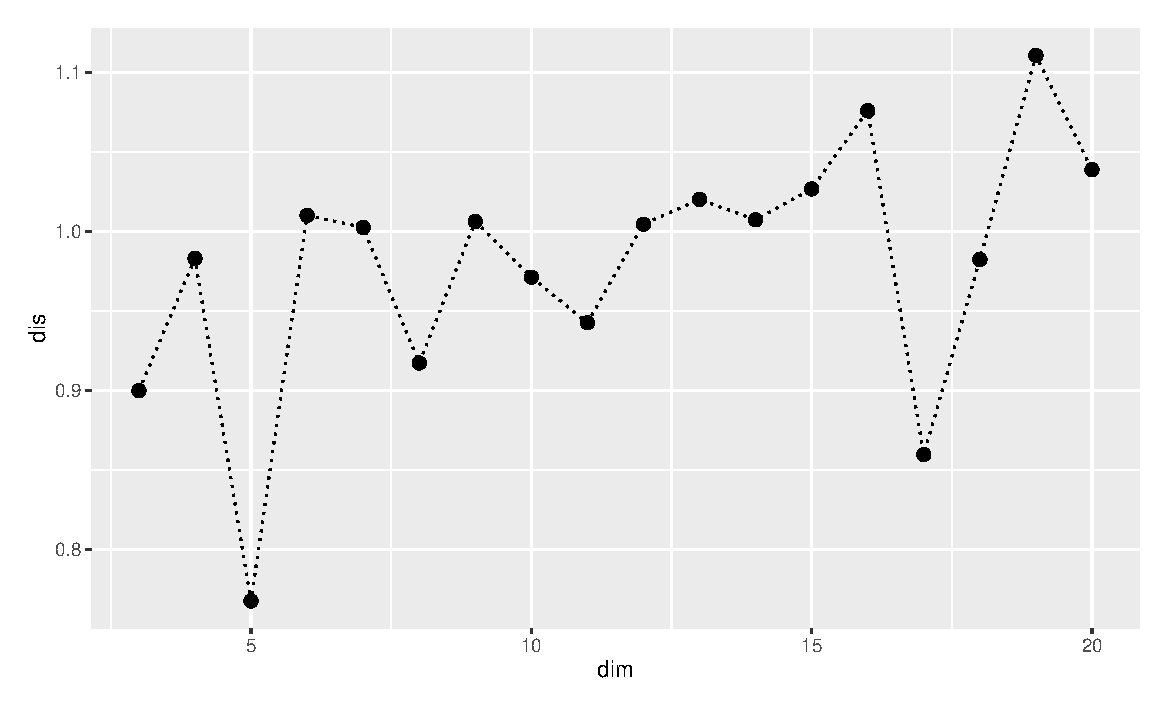
\includegraphics[width=0.8\textwidth]{image/pois_phd.eps}
    \caption{泊松回归下维度对降维效果的影响}
\end{figure}

\subsection{Logistic回归}

\begin{figure}[H]
    \centering
    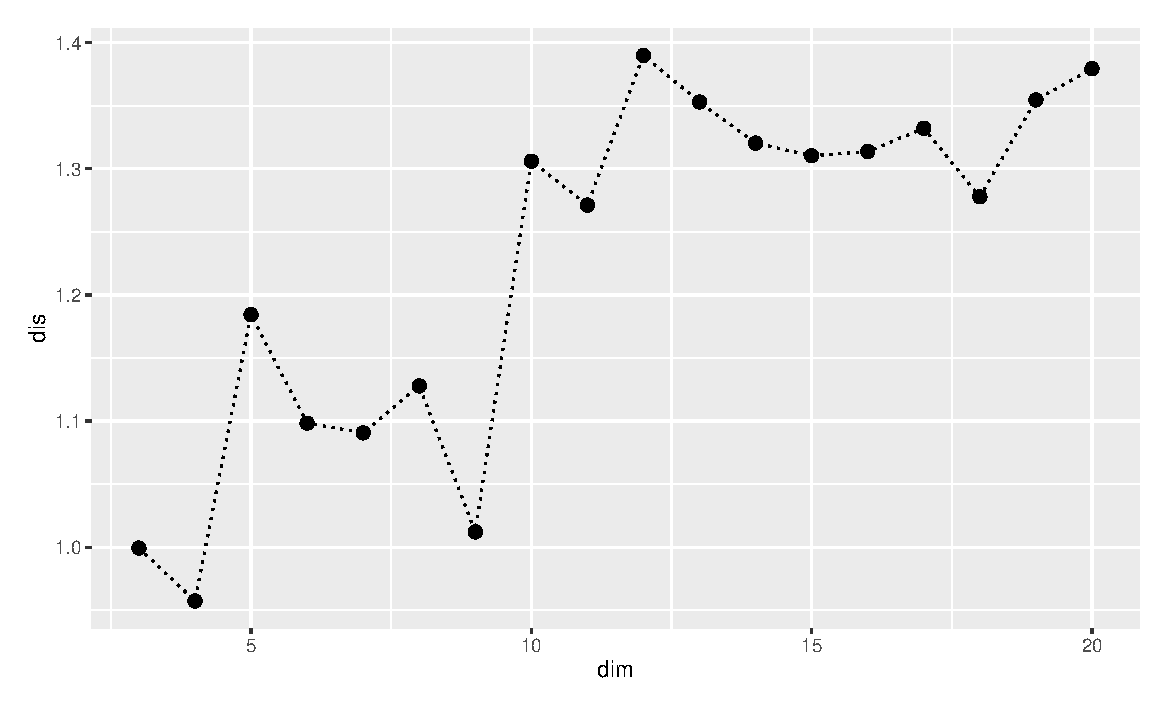
\includegraphics[width=0.8\textwidth]{image/logit_phd.eps}
    \caption{logistics回归下维度对降维效果的影响}
\end{figure}

\subsection{生成cos函数关系}
按$y=\cos(2\beta_1^Tx)+\cos(\beta_2^Tx)+\varepsilon$,生成样本y。其中$\beta_1$是参数矩阵$\beta$的第一列向量,同理$\beta_2$,而$\varepsilon$服从均值为0,方差0.1的正态分布。
\begin{figure}[H]
    \centering
    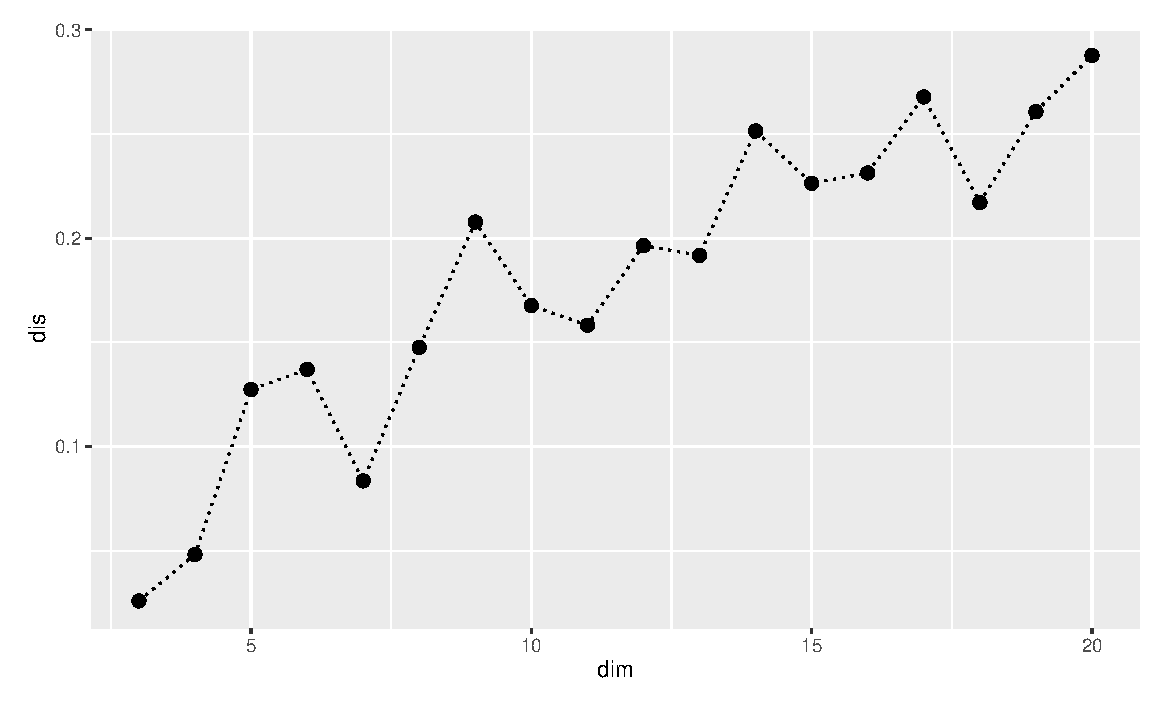
\includegraphics[width=0.8\textwidth]{image/cos_phd.eps}
    \caption{cos函数生成的数据下维度对降维效果的影响}
\end{figure}

\subsection{总结}
样本量始终为1000的情况下,且降维后的维度不变条件下,增大X的维数,估计空间与实际空间的差距呈上升趋势。而且实际上$L_2-Hausdorff$子空间距离最大值为子空间U和V的较大的维度的开根号,在实验中,即距离上限为$\sqrt{2}$,所以很明显这一方法在线性回归、Logistic回归以及Possion回归上的表现都不好,因为计算的$\beta$张成的空间的距离与pHd方法得到的估计张成的空间的距离是快达到上限的,仅在Y是X的cos相关函数的情况下效果较为理想。到20维距离也才为0.3,与0相近。但图像上还有些点显示出随维度上升距离反而还有下降的情况,


